
\definecolor{color1}{RGB}{77, 171, 247}
\definecolor{color2}{RGB}{132, 94, 247}
\definecolor{color3}{RGB}{255, 135, 135}
\definecolor{color4}{RGB}{11, 114, 133}
\definecolor{color5}{RGB}{59, 201, 219}
\definecolor{color6}{RGB}{132, 94, 247}

	
\begin{figure*}[t] %
     \vspace{-3mm}
    \centering %
    \resizebox{0.85\linewidth}{!}{  %
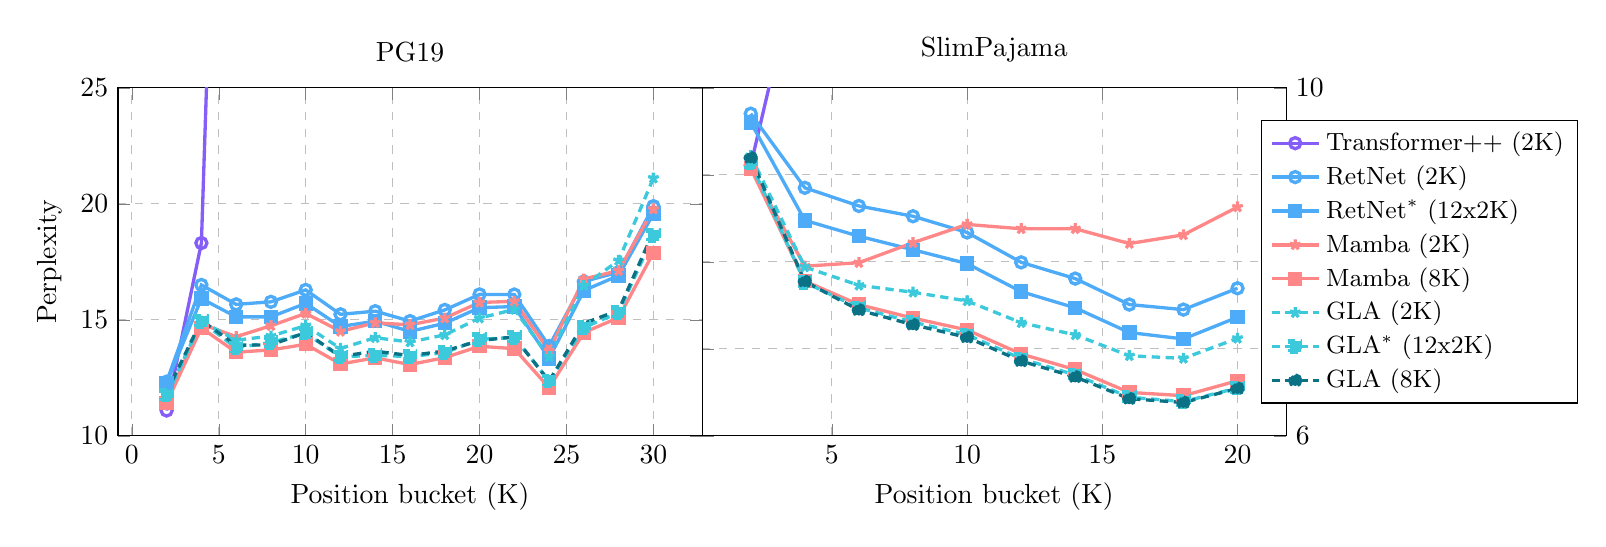
\begin{tikzpicture} %
        \scalefont{1.0} %
        \begin{axis}[
            name=plot1,
        sharp plot, %
        title style={align=right}, title={
        %
        PG19}
        ,
    %
			xmode=normal,%
%
			xlabel=Position bucket (K), %
			ylabel=Perplexity, %
			width=9cm, height=6cm,  %
			%
			ymin=10,
               ymax=25,  %
			%
                %
			%
			xlabel near ticks, %
			ylabel near ticks, %
			ymajorgrids=true, %
                xmajorgrids=true,
			grid style=dashed, %
			]
			%

\addplot+[very thick,mark=o,mark options={scale=1}, color=color6] plot coordinates { 
(2, 11.09)
(4, 18.31)
(6, 64.2)
};

%
\addplot+[very thick,mark=o,mark options={scale=1}, color=color1] plot coordinates { 
(2, 12.334416871694545)
(4, 16.50338878264782)
(6, 15.665969802718664)
(8, 15.775098093939631)
(10, 16.28891258448325)
(12, 15.237502382790032)
(14, 15.371704482324168)
(16, 14.94472773435605)
(18, 15.426467447568902)
(20, 16.095521862334422)
(22, 16.089831898143757)
(24, 13.870173108390853)
(26, 16.652435886300694)
(28, 17.05460165670472)
(30, 19.899968051899997)
};
			
%
\addplot+[very thick, mark=square*, mark options={scale=1}, color=color1] plot coordinates {
(2, 12.272513995002527)
(4, 15.915017718544624)
(6, 15.12648400208903)
(8, 15.126682357304789)
(10, 15.707573736739828)
(12, 14.711491336539076)
(14, 14.941795590117444)
(16, 14.499628795410947)
(18, 14.852281588773375)
(20, 15.52356082374071)
(22, 15.57131917875397)
(24, 13.332259116220783)
(26, 16.26334764613957)
(28, 16.90620689149074)
(30, 19.575600800473826)	
};

%
\addplot+[very thick,mark=star,mark options={scale=1}, color=color3] plot coordinates {
(2, 11.513764074464719)
(4, 14.821545167608454)
(6, 14.27181440333812)
(8, 14.745159645587211)
(10, 15.277090611163125)
(12, 14.503881505445126)
(14, 14.867072874125807)
(16, 14.785802233682734)
(18, 15.075549715264373)
(20, 15.74728691109622)
(22, 15.796882231799712)
(24, 13.665838224478483)
(26, 16.75761700477185)
(28, 17.122188320649027)
(30, 19.772022829026763)			
};

%
\addplot+[very thick,mark=square*,mark options={scale=1}, color=color3] plot coordinates {
(2, 11.420266254807174)
(4, 14.647489438851771)
(6, 13.602399098526789)
(8, 13.702136965988363)
(10, 13.94407030138506)
(12, 13.096784138731092)
(14, 13.358225399949397)
(16, 13.069880104168242)
(18, 13.369938037195737)
(20, 13.859198521307533)
(22, 13.75584104547106)
(24, 12.071451636850792)
(26, 14.451484019606044)
(28, 15.095705584933034)
(30, 17.893014429053675)	
};

%
\addplot+[very thick,mark=star,mark options={scale=1}, color=color5] plot coordinates {
(2, 11.688854804956376)
(4, 14.943035357330759)
(6, 14.119485985291082)
(8, 14.300316332465233)
(10, 14.748137591710703)
(12, 13.762720187004728)
(14, 14.227475231817666)
(16, 14.04244932822711)
(18, 14.34961326894769)
(20, 15.074579287890959)
(22, 15.446429587912565)
(24, 13.412177117829918)
(26, 16.474816040581416)
(28, 17.556498322948684)
(30, 21.106791888790198)	
};

%
\addplot+[very thick,mark=square*,mark options={scale=1}, color=color5] plot coordinates {
(2, 11.7457580111041)
(4, 14.920393773306506)
(6, 13.791731057875367)
(8, 14.025104116895617)
(10, 14.419469470911702)
(12, 13.408896666345553)
(14, 13.464048125083734)
(16, 13.417051316705868)
(18, 13.58252067910424)
(20, 14.157938178864061)
(22, 14.239108084631486)
(24, 12.368099123010358)
(26, 14.665233740423941)
(28, 15.31096912196873)
(30, 18.632639168708696)
};

%
\addplot+[very thick, mark= mark options={scale=1},  color=color4] plot coordinates {
(2, 11.872848224059455)
(4, 14.972456535259505)
(6, 13.906079604037489)
(8, 13.917668674699033)
(10, 14.450326377207194)
(12, 13.422948137513114)
(14, 13.644676392922488)
(16, 13.46075819589147)
(18, 13.653410626666675)
(20, 14.103521696916971)
(22, 14.265809961807271)
(24, 12.348204946403571)
(26, 14.846425830412182)
(28, 15.410869769068253)
(30, 18.799468389849164)
};

%
%
%
%
%
%
%
%
%
%
%
%
%
%
%
%
\end{axis}

\begin{axis}[
            name=plot2,
            at={(plot1.south east) },
        sharp plot, %
        title style={align=right}, title={
        %
        SlimPajama}
        ,
    %
			xmode=normal,%
%
			xlabel=Position bucket (K), %
			%
      ylabel near ticks, yticklabel pos=right,
			width=9cm, height=6cm,  %
			%
			%
   ymax=10,  %
   ymin=6,
			%
                %
			%
			xlabel near ticks, %
			ylabel near ticks, %
			ymajorgrids=true, %
                xmajorgrids=true,
			grid style=dashed, %
   			legend style={at={(1.5,0.5)},anchor=east,font=\small}, 
                legend cell align=left]
			%

			\addplot+[very thick,mark=o,mark options={scale=1}, color=color6] plot coordinates { 
(2, 9.11)
(4, 11.77)
%
%
%
%
%
%
%
%
};			
\addlegendentry{Transformer++ (2K)} ;

			\addplot+[very thick,mark=o,mark options={scale=1}, color=color1] plot coordinates { 
(2, 9.703324579039524)
(4, 8.851140172053045)
(6, 8.64224978739121)
(8, 8.523894072608067)
(10, 8.337787326052817)
(12, 7.993996058951587)
(14, 7.807283256053823)
(16, 7.508849714252663)
(18, 7.450385184846358)
(20, 7.696067587961978)			};
	\addlegendentry{RetNet (2K)};  
		
			%
			\addplot+[very thick, mark=square*, mark options={scale=1}, color=color1] plot coordinates {
(2, 9.60288660871554)
(4, 8.47661116643274)
(6, 8.294459081541115)
(8, 8.138966746337)
(10, 7.979737282823978)
(12, 7.65726433276238)
(14, 7.470669790601427)
(16, 7.187401744904839)
(18, 7.1132779884136905)
(20, 7.3631378999335295)		};
	\addlegendentry{RetNet$^*$ (12x2K) };  

			%
			\addplot+[very thick,mark=star,mark options={scale=1}, color=color3] plot coordinates {
(2, 9.07)
(4, 7.95)
(6, 7.99)
(8, 8.22)
(10, 8.43)
(12, 8.38)
(14, 8.38)
(16, 8.21)
(18, 8.31)
(20, 8.63)		};
	\addlegendentry{Mamba (2K) };  

   			\addplot+[very thick,mark=square*,mark options={scale=1}, color=color3] plot coordinates {
(2, 9.074799787988505)
(4, 7.7780675203930025)
(6, 7.508237473960171)
(8, 7.3529524666619945)
(10, 7.216372863755205)
(12, 6.940692359274163)
(14, 6.760323233107172)
(16, 6.49872027703192)
(18, 6.460961900906283)
(20, 6.6330331428715725)	};
	\addlegendentry{Mamba (8K) };  

\addplot+[very thick,mark=star,mark options={scale=1}, color=color5] plot coordinates {
(2, 9.22)
(4, 7.94)
(6, 7.73)
(8, 7.65)
(10, 7.55)
(12, 7.3)
(14, 7.16)
(16, 6.92)
(18, 6.89)
(20, 7.12)		};
\addlegendentry{GLA (2K) };  

\addplot+[very thick,mark=square*,mark options={scale=1}, color=color5] plot coordinates {
  (2, 9.134076157537933)
(4, 7.763725571624473)
(6, 7.470406185573722)
(8, 7.307020316318466)
(10, 7.162166118009677)
(12, 6.8859825063022155)
(14, 6.69981277659273)
(16, 6.443211499058021)
(18, 6.393198065692631)
(20, 6.54966772918719)
};
\addlegendentry{GLA$^{*}$ (12x2K) };  
\addplot+[very thick, mark options={scale=1},  color=color4] plot coordinates {
(2, 9.195530723286662)
(4, 7.773488412387971)
(6, 7.445253416398666)
(8, 7.276337205511129)
(10, 7.131082988866674)
(12, 6.858498031943685)
(14, 6.67630503682912)
(16, 6.426108888086446)
(18, 6.382840753376257)
(20, 6.543979086587886)
};
\addlegendentry{GLA (8K) };  
\end{axis}
\end{tikzpicture}
}
 \vspace{-3mm}
\caption{Length extrapolation on the test set of SlimPajama and  PG19. We pretrain 1.3B models from scratch on SlimPajama for 100B tokens with different training length. $^{\ast}$ indicates models using truncated BPTT with over 12 segments that are each of 2K-length.}
		\label{fig:length_extrapolate} 
     \vspace{-4.5mm}
	\end{figure*}

